%
% File acl2020.tex
%
%% Based on the style files for ACL 2020, which were
%% Based on the style files for ACL 2018, NAACL 2018/19, which were
%% Based on the style files for ACL-2015, with some improvements
%%  taken from the NAACL-2016 style
%% Based on the style files for ACL-2014, which were, in turn,
%% based on ACL-2013, ACL-2012, ACL-2011, ACL-2010, ACL-IJCNLP-2009,
%% EACL-2009, IJCNLP-2008...
%% Based on the style files for EACL 2006 by 
%%e.agirre@ehu.es or Sergi.Balari@uab.es
%% and that of ACL 08 by Joakim Nivre and Noah Smith

\documentclass[11pt,a4paper]{article}
\usepackage[hyperref]{acl2020}
\usepackage{times}
\usepackage{latexsym}
\renewcommand{\UrlFont}{\ttfamily\small}
\usepackage{booktabs}
\usepackage{tikz}
\usepackage{amsmath}
\usepackage{graphicx}

% This is not strictly necessary, and may be commented out,
% but it will improve the layout of the manuscript,
% and will typically save some space.
\usepackage{microtype}

%\aclfinalcopy % Uncomment this line for the final submission
%\def\aclpaperid{***} %  Enter the acl Paper ID here

%\setlength\titlebox{5cm}
% You can expand the titlebox if you need extra space
% to show all the authors. Please do not make the titlebox
% smaller than 5cm (the original size); we will check this
% in the camera-ready version and ask you to change it back.

\newcommand\BibTeX{B\textsc{ib}\TeX}

\title{Instructions for ACL 2020 Proceedings}

\author{First Author \\
  Affiliation / Address line 1 \\
  Affiliation / Address line 2 \\
  Affiliation / Address line 3 \\
  \texttt{email@domain} \\\And
  Second Author \\
  Affiliation / Address line 1 \\
  Affiliation / Address line 2 \\
  Affiliation / Address line 3 \\
  \texttt{email@domain} \\}

\date{}

\begin{document}
\maketitle
\begin{abstract}
  Basically we want to see if language models pre-trained on text data are useful for dialogue.
  So we look at if BERT is useful for dialouge act recoginiton.
  But we want to know if it's really adapting to the domain, so we look at how it uses laughter, a phenomenon specific to dialogue.
\end{abstract}

% INTRODUCTION

Recently, large-scale language models, trained on massive corpora of text data, have achieved state-of-the-art results on a variety of traditonal NLP tasks.
We investigate whether such models might be useful for processing dialogue, and if so, whether they adapt to make use of dialogue-specific features.

Dialogue, especially spoken dialogue, is radically different from the kind of data that neural language models are prestrained on.
Not only is the internal structure of contributions differ% - DA distribution              % Vlad
% - Laughter frequencies per DA  % Vlad

% - AMI, SWBD + comparison table % Bill
\begin{table}[]
\centering
\begin{tabular}{@{}ll@{}}
\toprule
\textbf{Switchboard}       & \textbf{AMI Corpus}                     \\ \midrule
Dyadic                     & Multi-party                             \\
Casual conversation        & Mock business meeting                   \\
Telephone                  & In-person \& video                      \\ \midrule
English                    & English                                 \\ 
Native speakers            & Native \& non-native speakers           \\ 
early '90s                 & 2000s                                   \\ \midrule
2200 conversations         & 171 meetings                            \\
  \hspace{1em} 1155 in SWDA               & \hspace{1em} 139 in AMI-DA                           \\
400 utterances             & 118k utterances                         \\
3M tokens                  & 1.2M tokens                             \\ \bottomrule
\end{tabular}
  \caption{Comparison between Switchboard and the AMI Meeting Corpus}
  \label{table:corpora}
\end{table}

% - Preprocessing: remove disfluencies, acronyms and speaker tokens in AMI, removing laughter % Bill
  
\section{Model} % Bill

Our DAR model has two components: an utterance encoder, and a sequence model that predicts the dialogue act tag (figure \ref{fig:model-architecture}).
Since we are primarily interested in comparing different utterance encoders, we use a simple RNN as the sequence model in every configuration. 
The RNN takes the encoded utterance as input at each time step
Its hidden state is passed to a simple linear classification layer over dilague act tags.
Conceptually, the encoded utterance represents the context-agnostic semantic content of the utterance, and the hidden state of the RNN represents the discourse context.

\begin{figure*}
  
\tikzstyle{rnn}=[rectangle,
  thick,
  minimum height=0.5cm,
  minimum width=2cm,
  fill=cyan]
\tikzstyle{encoder}=[rectangle,
  thick,
  minimum height=0.5cm,
  minimum width=2cm,
  fill=yellow]

\centering
\begin{tikzpicture}[>=latex,text height=1.5ex,text depth=0.25ex]
  \matrix[row sep=0.5cm,column sep=0.5cm] {
  % First line: Output labels
  \node (Y_0) []{$\hat{Y}_0$};&
  \node (Y_1) []{$\hat{Y}_1$};&
  \node (dots1) [] {$\dots$};  &
  \node (Y_T) []{$\hat{Y}_T$};&
  \\ % Second line: RNNs
  \node (RNN_0) [rnn]{RNN};&
  \node (RNN_1) [rnn]{RNN};&
  \node (dots2) [] {$\dots$};  &
  \node (RNN_T) [rnn]{RNN};&
  \\ % Third line: Linear layers
  \node (Encoder_0) [encoder]{Encoder};&
  \node (Encoder_1) [encoder]{Encoder};&
  \node (dots3) [] {$\dots$};  &
  \node (Encoder_T) [encoder]{Encoder};&
  \\ % Fourth line: Linear layers
  \node (Input_0) []{\small $ \underbrace{s^0,w^0_{0},w^0_{1},...,w^0_{n_0}}_{\text{Utterance 1}}$};&
  \node (Input_1) []{\small $ \underbrace{s^1,w^1_{0},w^1_{1},...,w^1_{n_1}}_{\text{Utterance 2}}$};&
  \node (dots4) [] {$\dots$};  &
  \node (Input_T) []{\small $ \underbrace{s^T,w^T_{0},w^T_{1},...,w^T_{n_T}}_{\text{Utterance T}}$};&
  \\ };
  \path[->]
  (Input_0) edge[thick]  (Encoder_0)	
  (Input_1) edge[thick] (Encoder_1)	
  (Input_T) edge[thick] (Encoder_T)	

  (Encoder_0) edge[thick] node[right] {} (RNN_0)	
  (Encoder_1) edge[thick] node[right] {} (RNN_1)	
  (Encoder_T) edge[thick] node[right] {} (RNN_T)	

  (RNN_0) edge[thick] (Y_0)	
  (RNN_1) edge[thick] (Y_1)	
  (RNN_T) edge[thick] (Y_T)	

  (RNN_0) edge[thick] node[above] {$h_1$} (RNN_1)
  (RNN_1) edge[thick] node[above] {$h_2$} (dots2)
  (dots2) edge[thick] node[above] {$h_T$} (RNN_T)
  ;
\end{tikzpicture}

  \caption{DAR model architecture}
  \label{fig:model-architecture}
\end{figure*}
%  - DAR model -> utt encoder, RNN sequence tagger
%  - BERT encoder (12 heads, uncased,...)
%  - baseline encoder

\section{Experiments}
\subsection{Experiment 1: Impact of laughter}   % Vlad
In the first experiment we investigated whether laughter, as an example of a dialogue-specific signal, is a helpful feature for DAR.
Therefore, we train another version of each model: one containing laughters (L) and with laughters left out (NL), and compare their performances in DAR task.
From the results (see Table~\ref{tab:laughter}) we can conclude that .
\begin{table}
  \label{tab:laughter}
  \centering
  \begin{tabular}{@{}lll@{}}
    \toprule
                      & SWDA  & AMI-DA \\ \midrule
    \texttt{BERT-NL}  & 77.07 & 67.06       \\ 
    \texttt{BERT-L}   & 76.93 & 67.12       \\ \midrule
    \texttt{CNN-NL}   & 75.08 & 63.46        \\
    \texttt{CNN-L}    & 75.40 & 64.30        \\ \bottomrule
    
  \end{tabular}
  \caption{Comparison of models depending on using laughter in training phase.}
\end{table}

\begin{figure*}
  \centering
  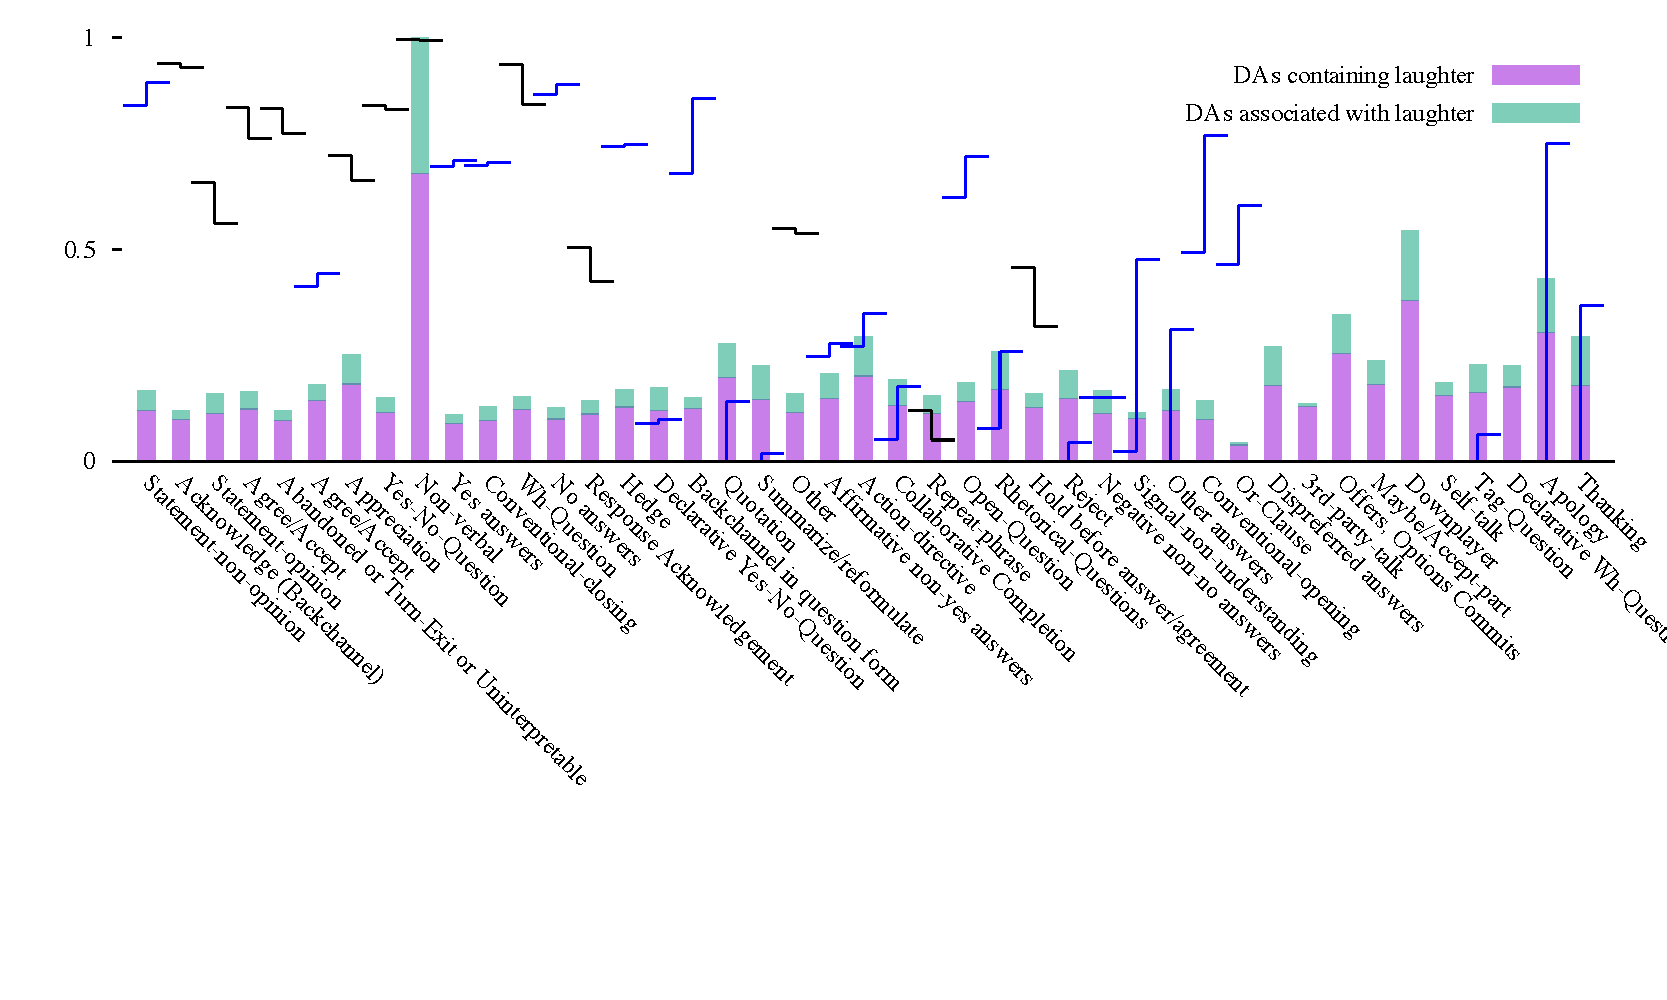
\includegraphics[width=\textwidth]{img/SWDA-bertLvsNL.pdf}
  \caption{Change in accuracy for each SWDA dialogue act. Positive changes when adding laughter are shown in blue. Vertical bars indicate how often dialogue act is associated with laughter.}
\end{figure*}

\begin{figure*}
  \centering
  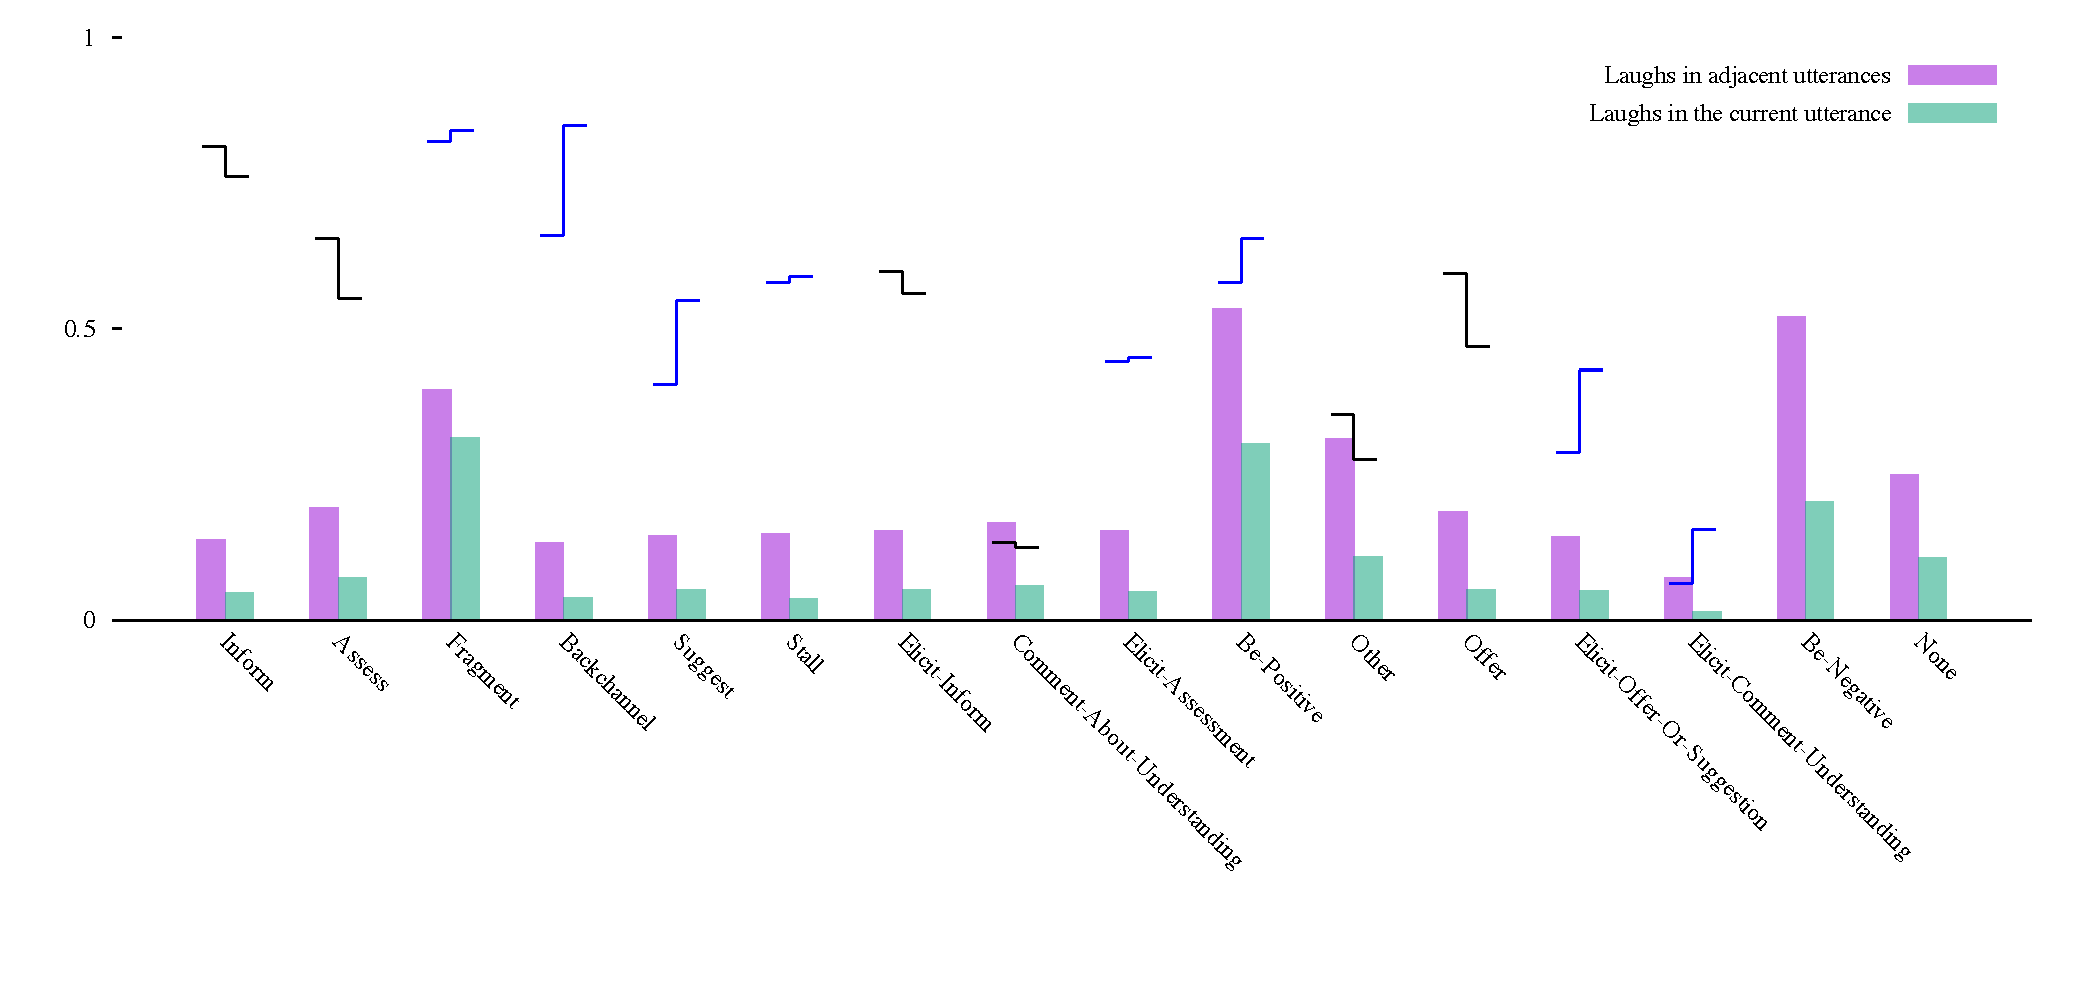
\includegraphics[width=\textwidth]{img/AMI-DA-bertLvsNL.pdf}
  \caption{Change in accuracy for each AMI dialogue act. Positive changes when adding laughter are shown in blue. Vertical bars indicate how often dialogue act is associated with laughter.}
\end{figure*}
% TODO per dialogue act analysis
% DONE compare impacts of CNN vs BERT
% DONE for both AMI and SWDA
% ? 

\subsection{Experiment 2: Impact of pre-training} % Bill
% - compare i) pre-trained BERT with freezing ii) pretrained with no freezing iii) randolmly initialized
Next, we take a direct look at how pre-training affects BERT's performance as an utterance encoder for our DAR model.
In particular, we consider the performance of DAR models with three different utterance encoders:
\begin{itemize}
  \item \texttt{BERT} -- pre-trained BERT without fine-tuning (frozen during DAR training)
  \item \texttt{BERT-FT} -- pre-trained BERT with fine-tuninig 
  \item \texttt{BERT-RI} -- randomly initialized BERT with fine-tuning 
\end{itemize}

\begin{table}[]
\centering 
\begin{tabular}{@{}lll@{}}
\toprule
                 & SWDA  & AMI-DA \\ \midrule
\texttt{BERT}       & 55.61 & 46.59  \\
\texttt{BERT-FT}    & 76.93 & 66.94  \\
\texttt{BERT-RI}    & 73.80 & 61.53  
\end{tabular}
  \caption{Micro-average DAR accuracy}
  \label{table:exp2-avg}
\end{table}    

The pre-trained model performs better than the randomly initialized model by several percentage points on both DA corpora (table \ref{table:exp2-avg}). 
These results suggest that BERT's extensive pre-training do provide some useful information for dialogue act recoginition.
However, we note that pre-training is not enough: the poor performance of the frozen \texttt{BERT} model indicates that fine-tuning is important for BERT's performance as an utterance encoder.
These observations raise two questions.
First, how does BERT's pre-training help with DAR? 
And second, in what way are the representations learned by pre-trained BERT lacking?
In other words, what is the contribution of fine-tuning?

To help answer these questions, we compare accuracy results of the above three models by dialogue act tag.

% TODO: add per dialogue act accuracy figures

\subsection{Experiment 3: Impact of dialogue pre-training} % Bill
% - pre-train AMI+SWBD -> train SWDA/AMI-DA -> test SWDA/AMI-DA
% - pre-traing tasks: 1) next utterance, 2) masked token, 3) both ?
% - compare frozen with no dialogue pre-training vs pre-trained on dialogue w.r.t. L/NL (same as in Experiment 1)
\begin{itemize}
  \item Setup
    \begin{itemize}
      \item we do additional pre-training for the BERT encoder on in-domain data
      \item note: this is sometimes referred to as fine-tuning, but we reserve that term for task-specific training of the encoder model

      \item SWDA/AMI (excluding dialogues in the DAR test set)
      \item 10 epoch AMI / 10 epochs SWBD / 5 epochs of each
    \end{itemize}
\end{itemize}

\subsection{Experiment 4: Cross-domain pre-training (if time permits)} % Bill
%  - cross-domain pre-training

\section{Discussion} % add items to discuss
\begin{itemize}
  \item RoBERTa training scheme finds that next sentence prediction is of little importance. Is this true for us too? (suspect not due to discourse importance). see: https://github.com/huggingface/transformers/issues/1622
\end{itemize}

\bibliography{acl2020}
\bibliographystyle{acl_natbib}

\end{document}
